\chapter{From Zero to a Money Game}

This chapter follows a School of Hard Knocks interview with Victor, curated for the LazyEarn track by LazyingArt LLC. The source is not a blackboard lecture with formal equations; it is an interview about wealth, business, attention, and operating judgment. Still, the interview has a mathematical spine: large outcomes are repeatedly broken into smaller units, repeated actions, and feedback loops. We will keep the claims source-conscious, distinguish anecdote from mechanism, and use the arithmetic only where the transcript supports it.

\section{The Opening Claim: From Zero to Eight Figures}

The interview opens by asking us to hold two facts in tension. Victor is introduced as someone who was down to zero dollars at 19, and who, by 26, is said to have a net worth over ten million dollars. In the interview's framing, the contrast is the setup:

\begin{equation}
N_{19} \approx 0,
\qquad
N_{26} > 10{,}000{,}000,
\end{equation}

where \(N_a\) denotes Victor's claimed net worth at age \(a\). This notation is not audited accounting; it is only a compact way to preserve the interview's numerical claim.

The first measured proof of current motion comes when Victor says he is halfway through the year and at six million. If we call that amount \(R_{\text{half-year}}\), then the transcript gives

\begin{equation}
R_{\text{half-year}} \approx 6{,}000{,}000.
\end{equation}

The title of the lecture points toward twelve million a year. The transcript itself supports this as a run-rate inference rather than a completed-year statement:

\begin{equation}
R_{\text{annualized}}
\approx 2R_{\text{half-year}}
\approx 2 \times 6{,}000{,}000
= 12{,}000{,}000.
\end{equation}

That is the first lesson in source discipline. We preserve the number because it matters, but we also preserve its status: Victor says six million halfway through the year; twelve million is the natural annualized reading if that pace continues.

\section{The First Mechanism: Weekly Drops and Attention}

The interview then narrows from the headline to the origin. James asks when Victor started his first business. Victor says he was 19, and the business was his clothing brand, an e-commerce apparel project.

The important move is not simply that he chose e-commerce. The important move is cadence. Asked how he stood out in a competitive apparel market, Victor does not describe a single perfect product launch. He describes dropping clothes every week, whether the drops were good, bad, or uncertain. The point was to stay in front of people.

We can summarize the mechanism as

\begin{equation}
\text{weekly drops}
+
\text{repeated exposure}
+
\text{feedback}
\longrightarrow
\text{distribution advantage}.
\end{equation}

This is not a formal law. It is a compact expression of the interview's operating claim: in a crowded social-media environment, waiting six months to perfect a project can be weaker than staying visible every week.

\subsection{Question \& Answer}

\paragraph{Question.}
Why might imperfect weekly drops beat a polished six-month launch?

\paragraph{Answer.}
Because the market is not only judging product quality; it is also allocating attention. Victor's answer is that no one is waiting six months for the next big project. Repeated drops keep the brand in front of customers, make the brand familiar, and let the creator learn faster. In that sense, the product is not only the clothing. The product is also the cadence of contact with the audience.

\begin{figure}[h]
\centering
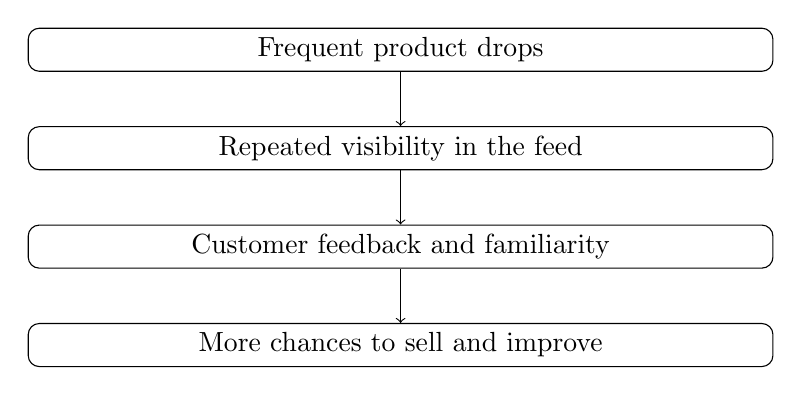
\begin{tikzpicture}
\node[draw, rounded corners, align=center, minimum width=0.78\linewidth] (a) at (0,0) {Frequent product drops};
\node[draw, rounded corners, align=center, minimum width=0.78\linewidth] (b) at (0,-1.25) {Repeated visibility in the feed};
\node[draw, rounded corners, align=center, minimum width=0.78\linewidth] (c) at (0,-2.50) {Customer feedback and familiarity};
\node[draw, rounded corners, align=center, minimum width=0.78\linewidth] (d) at (0,-3.75) {More chances to sell and improve};
\draw[->] (a) -- (b);
\draw[->] (b) -- (c);
\draw[->] (c) -- (d);
\end{tikzpicture}
\caption{The transcript-backed attention cadence: repeated releases create repeated contact with the market.}
\end{figure}

\section{Making a Million Smaller}

The next pivot is scale. James asks how Victor turned six figures into seven figures. Victor's answer is the central arithmetic of the interview: money is a game of numbers, and people are overwhelmed by the million-dollar figure because they see it as one object.

Victor compresses the arithmetic in speech. The intended structure is naturally read as

\begin{align}
10{,}000 \times 10 &= 100{,}000, \\
100{,}000 \times 10 &= 1{,}000{,}000.
\end{align}

The point is not that this alone produces a business. The point is psychological and operational. A million dollars becomes a sequence of repeated targets.

\begin{table}[h]
\centering
\begin{tabular}{c|c|c}
Target step & Unit & Repetitions \\
\hline
Reach \(100{,}000\) & \(10{,}000\) & \(10\) times \\
Reach \(1{,}000{,}000\) & \(100{,}000\) & \(10\) times \\
\end{tabular}
\caption{Victor's target decomposition, normalized from the transcript's compressed phrasing.}
\end{table}

\subsection{Question \& Answer}

\paragraph{Question.}
How does breaking the target into repeated units change the operator's behavior?

\paragraph{Answer.}
It shifts the problem from awe to procedure. A single million-dollar goal can freeze the beginner. Ten repetitions of a smaller unit can be scheduled, tested, and improved. The arithmetic does not remove the difficulty, but it changes the shape of the difficulty.

A worked version of the interview's reasoning is:

\begin{enumerate}
\item Start with the intimidating target:
\[
G = 1{,}000{,}000.
\]
\item Choose an intermediate unit:
\[
G = 10 \times 100{,}000.
\]
\item Decompose the intermediate unit again:
\[
100{,}000 = 10 \times 10{,}000.
\]
\item Therefore the million-dollar target can be viewed as nested repetition:
\[
1{,}000{,}000
=
10 \times (10 \times 10{,}000).
\]
\end{enumerate}

That is the chapter's small piece of mathematics. It is not advanced, but it is serious in the practical sense: it changes the operator's unit of action.

\section{Bootstrapping, Consistency, and Showing Up}

After the arithmetic, Victor immediately returns to behavior. He says that with team or no team, he did not use ads or a budget to propel the work. He describes the growth as bootstrapping and being in the field every day.

This is where the earlier formula must be read correctly. Repetition only matters if the operator actually repeats. We can write the practical update rule as

\begin{equation}
A_{t+1} = A_t + \Delta_{\text{visibility}} + \Delta_{\text{learning}},
\end{equation}

where \(A_t\) is not a formal account balance but a shorthand for accumulated audience position, market knowledge, and operating momentum at time \(t\). The transcript's word for this is simpler: consistency.

The key caution is that Victor is not giving a universal theorem against advertising. He is describing his own route: daily fieldwork and repeated market contact substituted for paid amplification.

\section{Sales as Pull, Not Push}

The interview then turns to sales. James asks what happens when a potential client or customer is on the fence and leaning toward no. Victor's answer is blunt: do not push.

The mechanism is social, not algebraic. Pushing too hard signals need. Need weakens the seller's position. Victor's preferred alternative is to become so good and so visible that people come to him, and then he can select who gets access. The later example is an elite program and a subscription that lets people enter the website earlier than everyone else.

In compact form:

\begin{equation}
\text{pressure selling}
\longrightarrow
\text{seller appears needy},
\end{equation}

whereas

\begin{equation}
\text{visible demand}
\longrightarrow
\text{selectivity}
\longrightarrow
\text{access product}.
\end{equation}

The sales lesson therefore extends the attention lesson. At first, weekly drops create visibility. At the sales stage, visibility becomes demand, and demand can be organized into access.

\section{Network, Rooms, and Mutual Exchange}

The next subject is relationships. Victor says that besides consistency, network is one of the most important things. The reason is environmental: if the room is too small, the person may mistake a local ceiling for a true ceiling.

The interview then raises a sharper problem. What does someone do if they do not yet know how to get into better rooms?

\subsection{Question \& Answer}

\paragraph{Question.}
How does a beginner enter better rooms without asking for help first?

\paragraph{Answer.}
Victor's answer is to invest in oneself until one has something to offer. The beginner should not enter the room with a hand out. The beginner should enter with a sharpened skill. If someone has more money or more success but lacks a capability, the beginner can fit like a missing piece.

\begin{figure}[h]
\centering
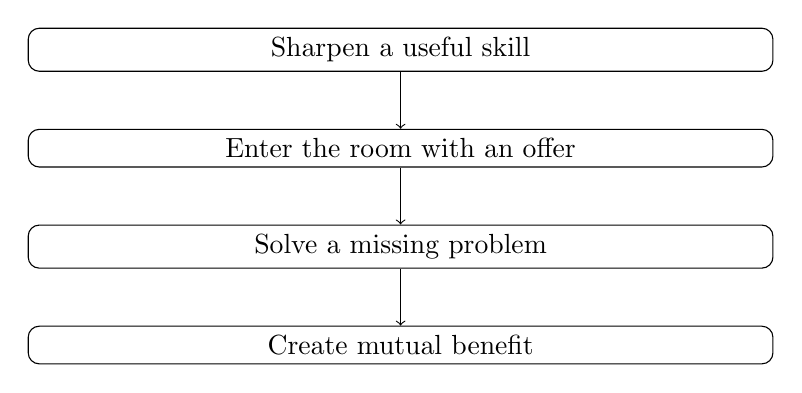
\begin{tikzpicture}
\node[draw, rounded corners, align=center, minimum width=0.78\linewidth] (a) at (0,0) {Sharpen a useful skill};
\node[draw, rounded corners, align=center, minimum width=0.78\linewidth] (b) at (0,-1.25) {Enter the room with an offer};
\node[draw, rounded corners, align=center, minimum width=0.78\linewidth] (c) at (0,-2.50) {Solve a missing problem};
\node[draw, rounded corners, align=center, minimum width=0.78\linewidth] (d) at (0,-3.75) {Create mutual benefit};
\draw[->] (a) -- (b);
\draw[->] (b) -- (c);
\draw[->] (c) -- (d);
\end{tikzpicture}
\caption{The relationship mechanism: network access is framed as exchange rather than extraction.}
\end{figure}

This is one of the interview's most useful distinctions. Networking is not treated as social climbing alone. It is treated as a matching problem between capability and need.

\section{Income Becomes Assets, Time Becomes Leverage}

James then asks for the best financial advice Victor has received. Victor credits Chris Johnson and gives a phrase that the transcript renders as ``get money by income.'' The phrase is probably compressed, but Victor immediately defines the meaning: whatever money you receive, use it to buy assets that make you more money.

The mechanism is clear enough to preserve:

\begin{equation}
\text{income}
\longrightarrow
\text{asset purchase}
\longrightarrow
\text{more income}
\longrightarrow
\cdots.
\end{equation}

This is the interview's wealth-conversion loop. Income alone is a flow. The advice is to turn part of that flow into ownership or control of assets that generate further flow.

\begin{figure}[h]
\centering
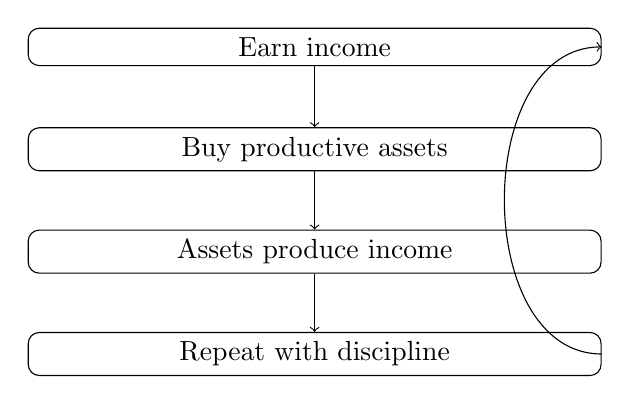
\begin{tikzpicture}
\node[draw, rounded corners, align=center, minimum width=0.60\linewidth] (a) at (0,0) {Earn income};
\node[draw, rounded corners, align=center, minimum width=0.60\linewidth] (b) at (0,-1.30) {Buy productive assets};
\node[draw, rounded corners, align=center, minimum width=0.60\linewidth] (c) at (0,-2.60) {Assets produce income};
\node[draw, rounded corners, align=center, minimum width=0.60\linewidth] (d) at (0,-3.90) {Repeat with discipline};
\draw[->] (a) -- (b);
\draw[->] (b) -- (c);
\draw[->] (c) -- (d);
\draw[->] (d.east) .. controls (2.0,-3.90) and (2.0,0) .. (a.east);
\end{tikzpicture}
\caption{The reinvestment loop described in the interview: received money is used to buy assets that can make more money.}
\end{figure}

The next question moves from money to mindset. Victor says the main habit is discipline and careful selection of what one uses time on. Time is worth more than money, he says, because wealth requires leverage over time. The temptation is to pick the easy, fun, attractive-looking thing. The work that compounds is often boring, consistent, and simple.

So the loop is not merely financial. It is also temporal:

\begin{equation}
\text{disciplined time}
\longrightarrow
\text{consistent action}
\longrightarrow
\text{accumulated advantage}.
\end{equation}

\section{Skill, Restart, and Legacy}

Near the end, the questions speed up. James asks for the most important skill for a young entrepreneur. Victor answers: social media marketing. In his view, social media is the catalyst for scaling from zero to a million because it gives access to attention.

Then James asks the restart question: if everything were taken and the bank account hit zero tomorrow, what would Victor do first? Victor's answer begins with network. He says he would call a friend, borrow ten grand, and run the play again. Then he would probably start a short-form service business, such as car detailing, to stack funds and keep his hands busy before moving back into digital real estate.

In source-conscious notation, the restart play looks like

\begin{equation}
0
\longrightarrow
\text{network trust}
\longrightarrow
10{,}000
\longrightarrow
\text{service cash flow}
\longrightarrow
\text{digital assets}.
\end{equation}

This is not a recommendation that every beginner can borrow ten thousand dollars. It is evidence for the earlier claim that network is part of the capital structure. Relationships are not just emotional support; in Victor's account, they can become financing, information, and opportunity.

The interview ends with legacy. Victor wants a wider reach and says that in five years he wants to be a household name, known for helping other people change their financial careers and learn business and entrepreneurship. The closing returns us to the opening: the money game is not described only as accumulation, but also as reach.

\section{Summary}

The interview's structure is simple but disciplined. It begins with a large claim, then walks backward into the mechanisms: a first e-commerce brand, weekly drops, social-media attention, target decomposition, bootstrapped consistency, pull-based sales, network as environment, value exchange, reinvestment, disciplined time, and social media marketing.

The main equations are not physics equations; they are practical arithmetic and mechanism diagrams. A million dollars becomes smaller when written as repeated units. Income becomes wealth only if some of it is converted into productive assets. Attention becomes distribution only if contact with the market is repeated.

The final lesson is not that Victor's path is mechanically reproducible for everyone. The source-conscious claim is narrower and stronger: in this interview, Victor explains his rise as a sequence of repeatable operating moves, each one turning a large vague goal into a smaller action that can be done again.